\documentclass[conference]{IEEEtran}

\usepackage{amsmath}
\usepackage{booktabs}
\usepackage{graphicx}
\usepackage{url}
\renewcommand{\UrlFont}{\rmfamily}

% TODO before submission: confirm the final author list with the supervisor.
% TODO before submission: the conference website gives conflicting instructions
% about double-blind review and author names; confirm whether anonymisation is required.

\title{Simulation-Grouped Per-Class QoS Prediction for SD-WAN}

\author{\IEEEauthorblockN{Radhika (Rishiv) Shitlani}
\IEEEauthorblockA{School of Computer Science\\
University of Galway, Galway, Ireland}}

\begin{document}

\maketitle

\begin{abstract}
Software-defined wide area networks (SD-WANs) must treat traffic classes differently, yet a single strong overall accuracy score can mask poor performance for the class that most needs scrutiny: best-effort traffic. This paper addresses two related tasks: predicting per-flow delay and detecting service-level-agreement (SLA) violations. We use 29,280 flow records from 400 BNNetSimulator runs, covering Gold, Silver, and Bronze traffic under three scheduling policies. An XGBoost regressor is evaluated with five-fold cross-validation grouped by simulation identifier, ensuring that no simulation run contributes flows to both sides of a fold. Under this grouped protocol, the model achieves an overall log-delay $R^2$ of 0.747, with class-specific values of 0.907, 0.898, and 0.680 for Gold, Silver, and Bronze; the corresponding SLA-violation F1 scores are 0.940, 0.680, and 0.554. A conventional row-wise split reports a higher $R^2$ of 0.766, consistent with modest optimism from shared simulation context across folds. The same grouped protocol shows that 90th-percentile delay is only moderately predictable ($R^2=0.293$ overall) and that jitter is not predicted reliably ($R^2=-0.040$). These results indicate that grouped, per-class evaluation is important for credible QoS prediction when multiple dependent flows originate from each simulation run.
\end{abstract}

\begin{IEEEkeywords}
SD-WAN, quality of service, machine learning, XGBoost, grouped cross-validation, SLA prediction
\end{IEEEkeywords}

\section{Introduction}

Software-defined wide area networking (SD-WAN) separates network control from packet forwarding, giving operators centralized control over routing and QoS policy across heterogeneous links. In practice, however, this control is typically exercised too late: operators adjust queue weights or reroute traffic only after congestion has already affected users. Predicting QoS ahead of an SLA breach could make this process proactive rather than reactive, but only if the prediction can be trusted for the traffic that most needs protecting. Gold, Silver, and Bronze traffic differ in priority, in how their delay behaves, and in what an error actually costs, so a model that appears accurate on average can still be unreliable for exactly the class most exposed to congestion.

Machine learning has already found several applications in SD-WAN research, including predicting how many virtual network functions a network will require~\cite{rahman2019autoscaling}, routing traffic based on application type~\cite{zheng2022applicationaware}, and steering traffic engineering with reinforcement learning~\cite{dinh2024safeloadbalancing,chen2025mteal}. Other work optimises SD-WAN routes and queueing policies directly from measured QoS~\cite{quang2022routing,quang2023globalqos}. These studies demonstrate that predictive or adaptive control is feasible, but none directly answer a narrower, more practical question: how accurately can continuous delay and SLA violations be predicted, separately for each traffic class, from a compact and reproducible feature set?

A second, less obvious problem is evaluation leakage. Each packet-level simulation run produces many flow rows at once, so randomly splitting individual rows can place flows from the same run on both sides of a train/validation split. The simulation identifier is never used as an input feature, but the shared topology, load, and scheduler conditions behind those rows can still make the validation task artificially easy. This paper therefore treats the simulation run, rather than the individual flow row, as the unit of evaluation.

This paper makes three contributions:
\begin{itemize}
    \item a reproducible per-class delay-prediction study using 29,280 flows from 400 BNNetSimulator runs;
    \item a simulation-grouped evaluation reporting both regression and SLA-trigger performance separately for Gold, Silver, and Bronze traffic, with row-wise cross-validation retained only as a sensitivity comparison; and
    \item an extension of the grouped protocol to two secondary QoS targets, tail (90th-percentile) delay and jitter, establishing the limits of what a static configuration feature set can predict.
\end{itemize}

\section{Related Work}

Machine learning has been applied to several adjacent network-management tasks, though rarely to per-class QoS prediction itself. Rahman \emph{et al.} predict how many virtual network functions a system will require as load changes~\cite{rahman2019autoscaling}, while Zheng \emph{et al.} combine traffic classification with QoS-aware routing decisions~\cite{zheng2022applicationaware}; both use machine learning to inform a decision rather than to predict a continuous QoS outcome per class. For SD-WAN specifically, Quang \emph{et al.} formulate joint routing and QoS policy optimisation~\cite{quang2022routing} and later add passive available-bandwidth estimation to a two-loop controller~\cite{quang2023globalqos}; these are optimisation systems built around a fixed queueing model rather than learned predictors evaluated against ground truth. Recent work also explores safe deep reinforcement learning for load balancing~\cite{dinh2024safeloadbalancing} and multi-objective, graph-based traffic engineering~\cite{chen2025mteal}. Among these reviewed studies, none reports how well delay or SLA compliance can be predicted separately for each priority class, which is the specific gap this paper addresses.

When labelled enterprise telemetry is unavailable, network simulators offer a reproducible alternative. BNNetSimulator generates packet-level data compatible with the modelling methodology behind RouteNet-Fermi~\cite{bnnupc2023bnnetsimulator,ferriolgalmes2022routenetfermi}, and this study uses it to examine a narrower, more practical question than the wider literature addresses: can static configuration and path features alone support reliable, class-specific QoS prediction? XGBoost is used as the primary model because gradient-boosted trees remain strong performers on small-to-medium tabular datasets~\cite{grinsztajn2022trees,shwartzziv2022tabular}, train comparatively quickly, provide inexpensive split-based feature-importance measures, and support efficient Tree SHAP explanations.

\section{Methodology}

\subsection{Dataset and QoS Classes}

The dataset was generated with the official BNNetSimulator container~\cite{bnnupc2023bnnetsimulator} and contains 29,280 source-destination flow records from 400 simulation runs, with 30--132 flows per run. Traffic is divided into three classes: Gold (4,592 rows, highest priority), Silver (8,991 rows, interactive traffic), and Bronze (15,697 rows, best effort). The experiments span strict priority, WFQ, and deficit round robin scheduling across four scenarios: fixed WFQ weights, randomised WFQ profiles, and two mixed-policy scenarios with skewed and equal class proportions. The generator was configured to avoid deliberate near-saturation, so the results below should be read as a controlled study of per-class prediction rather than a stress test of a saturated production network.

Each input row includes the traffic class, offered bandwidth, traffic distribution, route length, network size, maximum average load, link bandwidth, scheduling policy, class queue weight, and minimum class weight. The prediction target is the natural logarithm of average delay in seconds. Any field that would leak the answer, namely raw delay, jitter, packet loss, delay percentiles, achieved bandwidth, the scenario label, and the simulation identifier itself, is excluded from the feature matrix. Missing numeric values are median-imputed and categorical variables are one-hot encoded, both computed separately within each training fold to avoid leakage.

\subsection{Prediction and Grouped Evaluation}

The primary regressor is XGBoost, configured with 200 trees, a maximum depth of four, a learning rate of 0.05, and row and feature subsampling both set to 0.9. Because the model is trained on log delay, predictions are converted back to milliseconds before being reported, so that the error values carry operational meaning. Performance is measured using mean absolute error (MAE) on the millisecond scale and $R^2$ on log delay.

Five-fold cross-validation uses scikit-learn's GroupKFold with \emph{simulation\_id} as the grouping key, keeping every run's flows on one side of each fold. As a sensitivity check, the same model is also evaluated with a conventional shuffled, row-wise five-fold split, allowing the two protocols to be compared directly. Preprocessing and model fitting are refit independently within every fold.

Continuous delay predictions are also converted into binary SLA-violation triggers, using thresholds of 30, 50, and 60 ms for Gold, Silver, and Bronze respectively. Precision indicates how much a trigger can be trusted once it fires, recall indicates how many real violations are actually caught, and F1 balances the two. The Bronze threshold was derived from an exploratory sensitivity sweep rather than a fixed requirement, and should be read as a reasonable operating point rather than a universal SLA value.

The same grouped folds and leakage-safe feature exclusions are reused for two secondary targets, 90th-percentile delay and jitter, evaluated directly in milliseconds since that is the scale most relevant to the operational question. A negative $R^2$ in this context does not indicate an error; it indicates that the model's predictions generalise worse than simply predicting the validation-fold mean.

\subsection{Reproducibility}

Data generation, preprocessing, grouped evaluation, and plotting are implemented as separate, reusable Python scripts. Randomised estimators use a fixed seed (42), and every reported metric is derived from out-of-fold predictions rather than training predictions, ensuring that no result is inflated by the model having already seen the row it is scored on. The grouped evaluator also records which fold unit (row or simulation run) produced each result, to prevent the two from being conflated during reporting. The generated dataset, experiment scripts, and result tables are available in the project repository; a permanent archival identifier will be added for the camera-ready version.

\section{Results}

\subsection{Per-Class Delay and SLA Prediction}

Table~\ref{tab:grouped} reports the primary grouped results. Overall $R^2$ is 0.747, with a delay-scale MAE of 13.19 ms, though this single figure conceals a substantial class-dependent gap. Gold and Silver are predicted accurately ($R^2=0.907$ and 0.898), while Bronze falls to 0.680 and its MAE nearly triples to 21.57 ms. This pattern is consistent with protected traffic being shaped primarily by stable topology and scheduler configuration, which the static features capture well, while best-effort delay may also depend on transient contention that these features cannot observe.

\begin{table}[t]
\caption{Five-Fold Simulation-Grouped Results}
\label{tab:grouped}
\centering
\setlength{\tabcolsep}{3.5pt}
\begin{tabular}{lrrrrr}
\toprule
Class & MAE & $R^2$ & Prec. & Recall & F1 \\
 & (ms) & & & & \\
\midrule
Gold   & 3.17  & 0.907 & 0.986 & 0.898 & 0.940 \\
Silver & 3.67  & 0.898 & 0.798 & 0.593 & 0.680 \\
Bronze & 21.57 & 0.680 & 0.569 & 0.540 & 0.554 \\
\bottomrule
\end{tabular}
\end{table}

Gold's SLA trigger maintains a very high precision of 0.986: 98.6\% of predicted Gold violations are true violations (1,184 of 1,201). This is an important property for any controller that acts on such predictions, since false positives on the highest-priority class could trigger unnecessary intervention. Silver and Bronze are noticeably less reliable, particularly on recall, and Bronze's F1 of 0.554 illustrates an important point: a regressor that appears accurate in aggregate does not automatically translate into a strong SLA-violation detector for best-effort traffic.

\subsection{Effect of Grouping by Simulation}

Table~\ref{tab:protocol} and Fig.~\ref{fig:sensitivity} compare the grouped protocol against a conventional shuffled row-wise split. Grouping reduces overall $R^2$ from 0.766 to 0.747, with the largest drop occurring in Bronze, from 0.704 to 0.680, and its SLA F1 falling from 0.592 to 0.554; Gold is largely unaffected. This reduction is consistent with modest optimism from sharing simulation context across row-wise folds and supports treating the simulation run, rather than the row, as the evaluation unit for this dataset.

\begin{table}[t]
\caption{Sensitivity to the Cross-Validation Unit}
\label{tab:protocol}
\centering
\setlength{\tabcolsep}{4pt}
\begin{tabular}{lrrrr}
\toprule
Protocol & Overall & Gold & Silver & Bronze \\
 & $R^2$ & $R^2$ & $R^2$ & $R^2$ \\
\midrule
Row K-fold       & 0.766 & 0.914 & 0.908 & 0.704 \\
Grouped by run   & 0.747 & 0.907 & 0.898 & 0.680 \\
\bottomrule
\end{tabular}
\end{table}

\begin{figure}[t]
\centering
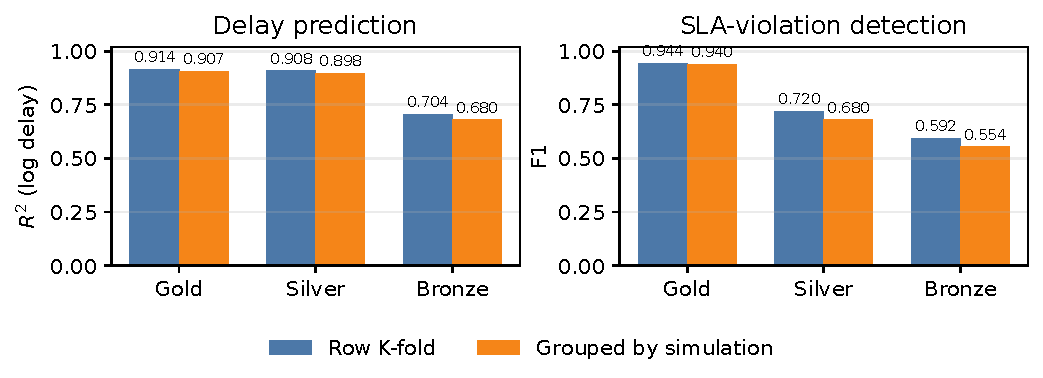
\includegraphics[width=\columnwidth]{figures/validation_sensitivity.pdf}
\caption{Row-wise and simulation-grouped performance by QoS class.}
\label{fig:sensitivity}
\end{figure}

An exploratory row-wise comparison found nearly identical overall scores for XGBoost ($R^2=0.766$), a multilayer perceptron (0.766), and an FT-Transformer (0.762). These neural results have not yet been repeated under simulation-grouped folds, so they are reported here only as supporting evidence rather than the paper's primary generalisation estimate, but they are sufficient to justify XGBoost as the lower-cost model of choice for the remainder of the study.

\subsection{Model Complexity and Feature Evidence}

Table~\ref{tab:models} breaks this exploratory comparison down by class. All three model families reach essentially the same Bronze ceiling under the row-wise protocol, and the FT-Transformer trails only marginally on Gold and Silver, with no gap exceeding 0.014 $R^2$. This is not proof of equivalence under grouped validation, but it is a clear signal that additional neural complexity provides little benefit here, since it cannot compensate for short-timescale traffic information absent from the feature set.

\begin{table}[t]
\caption{Exploratory Row-Wise Model Comparison}
\label{tab:models}
\centering
\setlength{\tabcolsep}{4pt}
\begin{tabular}{lrrrr}
\toprule
Model & Overall & Gold & Silver & Bronze \\
 & $R^2$ & $R^2$ & $R^2$ & $R^2$ \\
\midrule
XGBoost        & 0.766 & 0.914 & 0.908 & 0.704 \\
MLP            & 0.766 & 0.912 & 0.908 & 0.705 \\
FT-Transformer & 0.762 & 0.900 & 0.898 & 0.703 \\
\bottomrule
\end{tabular}
\end{table}

SHAP values for the final XGBoost model support this conclusion (Fig.~\ref{fig:shap}). Route length dominates: additional hops push predictions toward higher log delay, while shorter paths pull them down. Network size and traffic class follow at some distance, with queue weights and scheduling-policy indicators contributing comparatively little on their own. These represent associations learned within the simulator rather than causal estimates, but they tell a consistent story: the model relies primarily on stable path structure. This structure is genuinely informative for protected Gold and Silver flows, but the weaker Bronze results suggest that it does not fully capture transient contention affecting best-effort delay.

\begin{figure}[t]
\centering
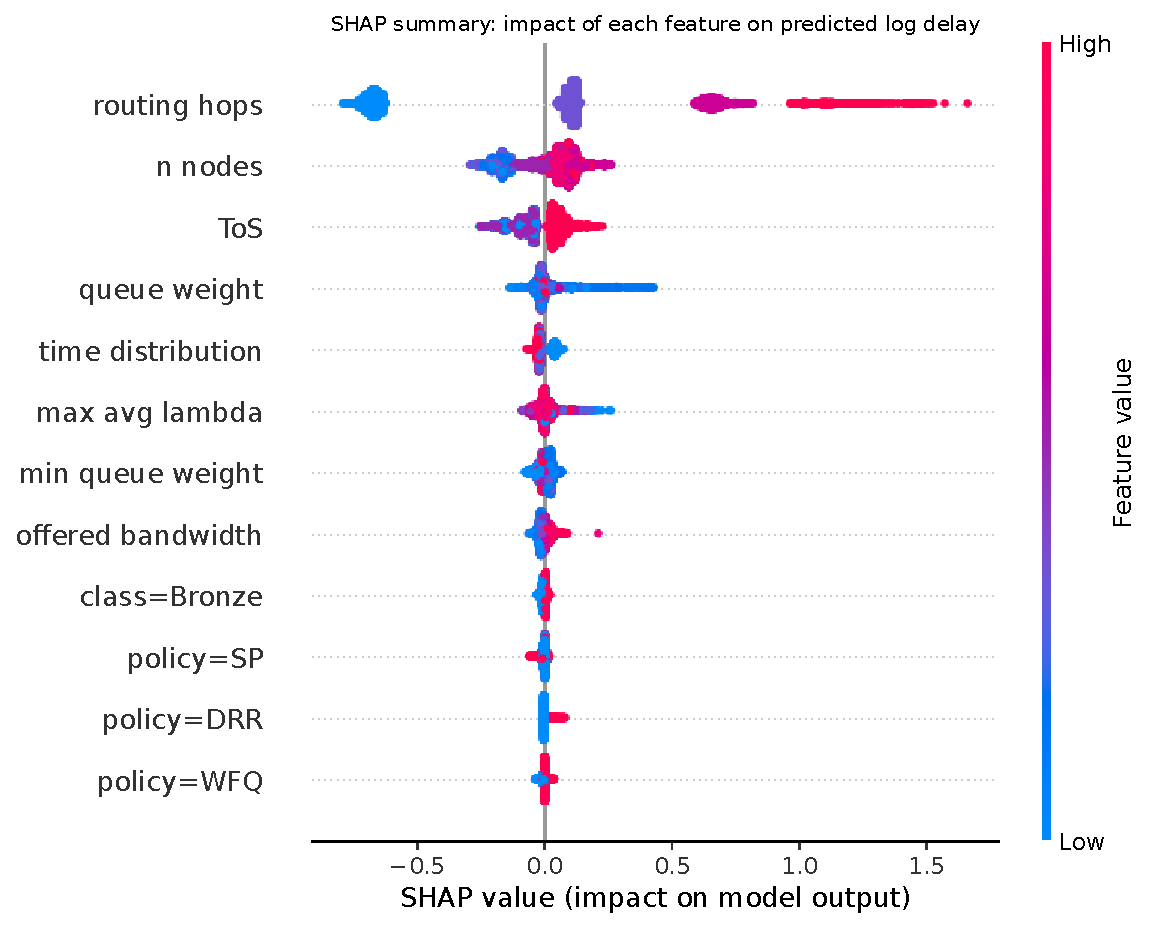
\includegraphics[width=0.95\columnwidth]{figures/shap_summary.pdf}
\caption{SHAP summary for the XGBoost log-delay model; colour denotes feature value.}
\label{fig:shap}
\end{figure}

\subsection{Tail Delay and Jitter}

Table~\ref{tab:secondary} applies the same grouped protocol to two secondary QoS targets. Tail delay is noticeably harder to predict than average delay: overall $R^2$ drops to 0.293, reaching only 0.550 and 0.490 for Gold and Silver, and falling further to 0.269 for Bronze, whose MAE climbs to 51.81 ms. This result is consistent with rare contention events influencing the upper tail, although those events are not directly measured by the current features.

Jitter does not generalise from the static feature set at all: overall $R^2$ is $-0.040$, and every class is negative. Gold and Silver exhibit small absolute MAE, but their within-class variance is so low that even modest errors exceed the error of simply predicting the validation-fold mean. Together, these results clarify the boundary of what this feature set can convey: it describes average delay well, tail delay only partially, and moment-to-moment delay variation not at all.

\begin{table}[t]
\caption{Grouped Results for Secondary QoS Targets}
\label{tab:secondary}
\centering
\setlength{\tabcolsep}{5pt}
\begin{tabular}{llrr}
\toprule
Target & Class & MAE (ms) & $R^2$ \\
\midrule
Delay p90 & Overall & 32.51 & 0.293 \\
          & Gold    & 8.92  & 0.550 \\
          & Silver  & 10.87 & 0.490 \\
          & Bronze  & 51.81 & 0.269 \\
\midrule
Jitter    & Overall & 3.22 & $-0.040$ \\
          & Gold    & 0.51 & $-7.555$ \\
          & Silver  & 1.01 & $-13.182$ \\
          & Bronze  & 5.28 & $-0.034$ \\
\bottomrule
\end{tabular}
\end{table}

\section{Discussion and Limitations}

The central finding here is not simply that delay is predictable, but that its predictability depends on the traffic class, the target, and the validation design employed. Route length, network size, and traffic class encode stable structure, and this structure explains protected average delay well. Bronze, having the lowest service priority, may be more exposed to bursts and queue occupancy that the current features do not measure. The poor jitter results reinforce this interpretation: increasing model complexity cannot recover transient state that is absent from the features.

Several limitations should temper these claims. First, the data is simulator-generated and was configured without deliberate near-saturation; grouped folds test generalisation to unseen runs from the same generator, not transfer to a real enterprise SD-WAN. Second, the feature set is entirely static: telemetry such as instantaneous queue occupancy, recent arrival-rate windows, and recent loss would be required to model transient behaviour, and none of this is present here. Third, the SLA thresholds used are experimental operating points rather than contractual values drawn from a real deployment. Future work should repeat every model comparison under grouped outer folds, evaluate under heavier congestion, and validate against real controller telemetry.

\section{Conclusion}

This paper presented a simulation-grouped, per-class evaluation of QoS prediction for SD-WAN-like networks. XGBoost generalises well to unseen simulation runs for Gold and Silver average delay, is noticeably less reliable for Bronze, and does not predict jitter reliably. In this dataset, row-wise cross-validation produces modestly higher scores than simulation-grouped validation, supporting the use of the simulation run rather than the individual flow as the evaluation unit. The broader implication is straightforward: trustworthy AI-assisted QoS prediction requires class-aware metrics, group-safe validation, and an honest account of what static network features can and cannot support.

\IEEEtriggeratref{3}
\bibliographystyle{IEEEtran}
\bibliography{references}

\end{document}
